\chapter{International Comparisons of Recidivism}

A recidivism rate standing by itself cannot be evaluated with respect to its magnitude.  Meaningful judgments concerning a particular recidivism rate require reference to recidivism rates drawn from other suitably comparable populations.  A comparative analysis of international recidivism rates furnishes this necessary basis for evaluative purposes.  The primary objective of this chapter is to determine how the recidivism rate for the United States compares with the recidivism rates of several similar countries.  The assessment of the recidivism rate for the United States will be useful for developing a sense of where Utah stands in comparison to the nation when Utah's recidivism rate, as derived from the Utah parolee data, is discussed in a subsequent chapter.

A question of considerable interest, particularly with respect to the formation of criminal justice policy, is whether there are any relationships among the crime, incarceration, and recidivism rates.  In addition to recidivism rates, crime and incarceration rates were collected for all of the countries selected for the international comparisons.  Two relationships were examined:  the relationship between recidivism and incarceration rates and the relationship between crime and incarceration rates.  In each case, the relationship is found to differ from intuitive expectations and raises important questions regarding criminal justice policy in the United States.

Upon examination of the international recidivism, crime, and incarceration rates and the relationships among these rates, the United States is evaluated relative to the other countries in the comparisons.  Viewing the statistics for the United States through the lens of international comparisons, it is evident that the purpose and efficacy of criminal justice policy in the United States is in need of critical reexamination.

\section[Recidivism in the United States and abroad]{Recidivism in the United States\\ and abroad}

For a comparative analysis to yield useful information, the populations under consideration must be reasonably similar.  In light of the fact that the recidivism rate for the United States is the central concern, the countries selected for comparison should share certain essential characteristics with the United States.  Among these characteristics, those of greatest importance are the legal system, the type of government structure, the level of economic development, and the cultural background.  In addition to sharing a set of requisite attributes, the countries under consideration must, of course, publish studies on recidivism.  These two criteria served to determine the selection of the countries for comparison with the United States.

The natural candidates for comparison with the United States include Australia, Canada, New Zealand, and the countries of Europe.  Australia, Canada, and New Zealand satisfied the two criteria and were included.  However, only a relatively small number of the European countries were included because of the absence of national recidivism statistics.  In a survey conducted by Wartna and Nijssen (2006), questionnaires were sent to 41 European countries, including Russia, inquiring about large-scale recidivism research.  Of the 33 countries that responded to the questionnaire, only 14 reported the existence of large-scale national studies on recidivism.  Even though the United Kingdom is typically viewed as a single political entity, the survey counted England and Wales, Northern Ireland, and Scotland as three individual countries.  Of the 14 countries reporting the presence of national recidivism studies, only Norway was excluded due to the unavailability of crucial information regarding the nature of sentenced offenders.  Thus, 13 European countries were selected for inclusion in the comparisons.  The complete list of countries selected for the international comparisons along with the sources of their recidivism rates is given as follows:  Australia (Jones, Hua, Donnelly, McHutchinson \& Heggie, 2006; Payne, 2007), Austria (Statistics Austria, 2008), Canada (Bonta, Dauvergne \& Rugge, 2003), Denmark (Denmark Department of Prisons and Probation, 2006), England/Wales (Spicer \& Glicksman, 2004), Finland (Hyp\'{e}n, 2003), France (Kensey \& Tournier, 2004, 2005), Germany (Jehle, Heinz \& Sutterer, 2003; Jehle, 2005), Iceland (Baumer, Wright, Kristinsdottir \& Gunnlaugsson, 2002), Ireland (O'Donnell, Baumer \& Hughes, 2008), the Netherlands (Wartna, Tollenaar \& Essers, 2005), New Zealand (Nadesu, 2007, 2008, 2009; New Zealand Department of Corrections, 2005), Northern Ireland (Ruddy \& Brown, 2008), Scotland (Scottish Executive, 2005), Sweden (National Council for Crime Prevention, 2008), Switzerland (Storz, 1997), and the United States (Langan \& Levin, 2002).

International comparisons of any type are always open to criticism on the basis that no two countries ever share enough of the necessary qualities to allow for valid comparative inferences. This view is likely correct in at least some cases.  An equally strong case, however, could be made that all of the selected countries have economic, political, and cultural institutions that are quite similar to those in the United States.  For the purpose of developing a general sense of where the United States stands relative to other countries in terms of recidivism, crime, and incarceration rates, the comparisons appear reasonable.

Aside from the issue of the similarity of the countries under comparison, another potentially troublesome issue is the comparability of the reported statistical figures.  No single, standardized approach to the collection, analysis, and publication of recidivism statistics is used by all of the countries selected for this comparison.  As a result, the differences in the statistics published by each country require a few qualifying remarks before any sound comparisons can be made.  These qualifications are fully addressed below.

\begin{sidewaystable}
\begin{center}
\caption{Reconviction Rates for the Selected Countries}
\vspace{0.1cm}
\small
\begin{tabular}{lrr@{,}lrcrrccccc}
  \hline
  % after \\: \hline or \cline{col1-col2} \cline{col3-col4} ...
  & \multicolumn{1}{c}{Release} & \multicolumn{2}{c}{} & \multicolumn{1}{c}{Age} & Crime & \multicolumn{2}{c}{Incarceration} & \multicolumn{5}{c}{Follow-up Periods in Years} \\ \cline{9-13}
  Country & \multicolumn{1}{c}{Period}  & \multicolumn{2}{c}{N} & \multicolumn{1}{c}{Range} & $\mbox{Rate}^a$ & \multicolumn{2}{c}{$\mbox{Rate}^b$} & 1 & 2 & 3 & 4 & 5  \\ \hline
  \vspace{0.1cm} Australia & 2001-2002 &  2 & 793 & 18 and up & 4,738 & 119 & &   &   & 63.9 &  &  \\
  \vspace{0.1cm} Austria & 2003 & 4 & 885 & 18 and up & 4,745 & \hspace{0.82cm} 96 & & 20.7 & 38.4 & 49.4 & 55.5 & 59.8 \\
  \vspace{0.1cm} Canada  & 1994-1997 & 14 & 306 & 18 and up & 5,074 & 114 & & & 42.9 & & & \\
  \vspace{0.1cm} Denmark &      2003 &  7 & 141 & 15 and up & 5,594 & 67  & & & 37.7 & & & \\
  \vspace{0.1cm} Finland &      1996 &  3 & 680 & 15 and up & 4,420 & 66  & & 15.1 & 32.1 & 42.1 & 48.2 & 52.2  \\
  \vspace{0.1cm} France  & 1996-1997 &  2 & 408 & 13 and up & 4,132 & 96  & & & & & & 51.9   \\
  \vspace{0.1cm} Germany &      1994 & 22 & 816 & 14 and up & 4,308 & 99  & & & & & 59.5 &  \\
  \vspace{0.1cm} Iceland & 1994-1998 &  1 & 176 & 18 and up & 2,328 & 38  & & 11.0 & 25.0 & 37.0 & 44.0 & 53.0 \\
  \vspace{0.1cm} Ireland & 2001-2004 & 19 & 955 & 15 and up & 2,578 & 81  & & 27.4 & 39.2 & 45.1 & 49.2 & \\
  \vspace{0.1cm} Netherlands & 1996-1999 & 69 & 602 & 18 and up & 5,758 & 100 & & 43.4 & 55.5 & 61.9 & 66.0 & 69.0 \\
  \vspace{0.1cm} New Zealand & 2002-2003 & 4 & 945 & 18 and up & 5,789 & 155 & & 42.6 & 55.4 & 62.0 & 68.0 & 70.8 \\
  \vspace{0.1cm} Sweden  & 2002-2005 & 13 & 958 & 15 and up & 8,214 & 75  & & & & 61.0 & & \\
  \vspace{0.1cm} Switzerland & 1988 & 6 & 393 & 18 and up & 4,125 & 71 & & 12.3 & 25.5 & 33.8 & 39.7 & 44.5  \\
  \vspace{0.1cm} UK: England \& Wales & 2001 & 14 & 569 & 18 and up & 7,414 & 140 & & & 58.2 & & & \\
  \vspace{0.1cm} UK: N. Ireland & 2004 & \multicolumn{2}{r}{825} & 17 and up & 4,684 & 68 & & 21.0 & 44.0 & & & \\
  \vspace{0.1cm} UK: Scotland & 1999 & 5 & 738 & 16 and up & 5,071 & 131 & & 46.0 & 60.0 & 67.0 & 71.0 &  \\
  \vspace{0.1cm} USA   & 1994 & 33 & 796 & 18 and up & 5,018 & 715 & & 21.5 & 36.4 & 46.9 & &  \\
  \hline
\end{tabular}
\vspace{0.1cm}

%\parbox{19.15cm}{\emph{Sources}: Baumer et al., 2002; Bonta, Dauvergne \& Rugge, 2003; Catalano, 2004; Department of Prisons and Probation, 2006; Harrison \& Karberg, 2004; Hyp\'{e}n, 2003; Jehle, Heinz \& Sutterer, 2003; Kensey \& Tournier, 2004; Langan \& Levin, 2002; National Council for Crime Prevention, 2008; O'Donnell, Baumer, \& Hughes, 2008; Ruddy \& Brown, 2008; Scottish Executive, 2005; Spicer \& Glicksman, 2004; Statistics Austria, 2008; Statistics Norway, 2007; Storz, 1997; United Nations, 2007; Wartna et al., 2005; WODC, 2006.}

\vspace{0.1cm}

\parbox{19.15cm}{\emph{Note.}  The rates reported for Finland and Ireland are reincarceration rates.}

\parbox{19.15cm}{$^a$Per 100,000 population, based on totals for intentional homicide, assault, rape, robbery, and theft for 2003.}

\parbox{19.15cm}{$^b$Per 100,000 population for 2003.}
\normalsize
\end{center}
\end{sidewaystable}


The recidivism statistics for the 17 countries are reported in Table 3.1.  The measure of recidivism used is the reconviction rate because it is the most widely available statistic.  However, only the reincarceration rates were available for Finland and Ireland.  Instead of omitting these countries from the comparisons, the decision was made to include their reincarceration rates and interpret them as the minima of the possible ranges of the reconviction rates.  In reference to Ireland's recidivism statistics, O'Donnell, Baumer, and Hughes (2008) argue that the reincarceration rate should be close to the reconviction rate because offenders with prior convictions are more likely to receive prison sentences upon reconviction (p. 128).  While arguments can be made for the inclusion or exclusion of Finland and Ireland from the comparisons, the decision was to include the statistics and leave it to the reader to choose whether or not to ignore those particular countries.

Another issue that creates some difficulty regarding comparability is the variation in the number of follow-up periods.  A few countries (e.g., the Netherlands and Finland) reported statistics for as many as eight follow-up periods, while some countries (e.g., Canada and Denmark) reported a recidivism statistic for only a single follow-up period.  The number of follow-up years in Table 3.1 was limited to five, even though some countries reported statistics beyond 5 years.  The variation in the number of follow-up years does create some uncertainty about the exact values of the rates for those years where they are unreported.  Nevertheless, there are generally enough rates reported for each of the follow-up years to allow for useful comparisons.

Of the five Nordic countries, only Norway's recidivism rate is not reported.  Even though Norway has conducted a large-scale recidivism study (Statistics Norway, 2007), one crucial figure was omitted in their statistics: the number of offenders released from a custodial sentence.  Thus, it was impossible to determine if individuals were released from custodial sentences or received other types of sentences.  Consequently, Norway was excluded.  As for the 17 countries included in Table 3.1, all of the offenders were released from custodial sentences.

One last caveat concerns the statistics for Scotland.  An examination of Table 3.1 reveals that Scotland has the highest reconviction rate in each of 4 follow-up years as compared to all of the other 16 countries.  However, the Scottish statistics contain a major flaw.  A significant number of individuals were counted as reconvicted for offenses that were committed prior to their initial prison release.  The 2-year rate is judged to be overstated by as much as 10\%, but no information is provided regarding the estimated overstatement for any other year, which makes correcting the rates impossible.  The rates found in Table 3.1 are the unadjusted rates taken as reported by the Scottish Executive (2005, Table 6, p. 10).

Before drawing a comparison between the United States and the other 16 countries, a few comments concerning the recidivism statistics for the United States are in order.  Two large-scale recidivism studies conducted by the U.S. Department of Justice's Bureau of Justice Statistics serve as the primary references for the recidivism statistics of the United States.  Beck and Shipley (1989) conducted the first study following 108,580 individuals released from prisons in 11 states in 1983.  In a more recent study, Langan and Levin (2002) followed 272,111 individuals released from prisons in 15 states in 1994, which represents approximately two-thirds of all releases from prison in 1994.  In both studies, the statistics were calculated using samples taken from the total number of released prisoners tracked.  On the whole, the two studies are remarkably similar.  In Table 3.2, three measures of recidivism are compared for the release years of 1983 and 1994.  The reincarceration rates listed in Table 3.2 are based on new convictions, not technical violations.  If technical violations are included, the 3-year reincarceration rate for prisoners released in 1994 is 51.8\%.  The reconviction rates for each year show no statistically significant differences. Because the reconviction rates are nearly the same in both studies and the 1994 study uses a larger, more recent data set, the reconviction rates reported in Table 3.1 were based on the results produced by Langan and Levin.



\begin{table}[b]
\begin{center}
\caption{United States Recidivism Rates for 1983 and 1994}
\vspace{0.1cm}
\begin{tabular}{ccccccccc}
  \hline
  % after \\: \hline or \cline{col1-col2} \cline{col3-col4} ...
   & \multicolumn{2}{c}{Rearrests} & & \multicolumn{2}{c}{Reconvictions} & & \multicolumn{2}{c}{Reincarcerations} \\ \cline{2-3} \cline{5-6} \cline{8-9}
  \mbox{Follow-up Years} & 1983 & 1994 & & \hspace{0.08cm} 1983 & 1994 & & \hspace{0.18cm} 1983 & 1994 \\ \hline
  1 & 39.3 & 44.1 & & \hspace{0.08cm} 23.1 & 21.5 & & \hspace{0.18cm} 18.6 & 10.4 \\
  2 & 54.5 & 59.2 & & \hspace{0.08cm} 38.3 & 36.4 & & \hspace{0.18cm} 32.8 & 18.8 \\
  3 & 62.5 & 67.5 & & \hspace{0.08cm} 46.8 & 46.9 & & \hspace{0.18cm} 41.4 & 25.4 \\
  \hline
\end{tabular}
\end{center}
\end{table}



Turning to the comparison between the United States and the other 16 countries, it must be concluded that the United States compares favorably.  The United States' ranking relative to the other countries is best appreciated by directly comparing the reconviction rates in the United States with the averages for all 17 countries.  The average international reconviction rates were formed by summing the rates for all of the countries that reported a rate during a particular follow-up year and dividing by the number of reported rates.  This method of forming the international average was chosen over a weighted-average based on the number of observations in each country's statistics because the populations and sample sizes tended to vary widely from country to country and the desire was to give each country the same overall weight.  It was previously mentioned that the recidivism measures for Finland and Ireland are reincarceration rates and that Scotland's reconviction rates included reconvictions for crimes committed prior to the most recent release.  The former statistics will tend to be underestimates of the true reconviction rates for each of the two countries, while Scotland's reconviction rates are overestimated.  Taken together, they will tend to offset each other.  On the whole, the international averages appear to be reasonable.

Table 3.3 directly compares the average for all 17 countries with the United States for the first 3 follow-up years.  The table reveals that the reconviction rate for each of the 3 follow-up years for the United States is approximately five percentage points lower than the average of the 17 countries.  While the United States does not have the lowest recidivism rates in the comparisons, they are lower than those of most countries.

\begin{table}[b]
\begin{center}
\caption{The International Average and U.S. Reconviction Rates}
\vspace{0.1cm}
\begin{tabular}{lccc}
  \hline
  % after \\: \hline or \cline{col1-col2} \cline{col3-col4} ...
  \mbox{Follow-up Periods in Years} & 1 & 2 & 3  \\ \hline
  \mbox{Average of International Reconviction Rates} & 26.1 & 42.3 & 51.8 \\
  \mbox{United States Reconviction Rates} & 21.5 & 36.4 & 46.9 \\
  \hline
\end{tabular}
\end{center}
\end{table}

Two last points deserve mention before turning to the examination of the relationships among international recidivism, crime, and incarceration rates.  First, it is of some interest to note how some pairs of countries that appear rather similar in terms of their economic, political, and cultural attributes have very different recidivism rates.  For example, the two Scandinavian countries of Iceland and Sweden share many of the same economic, political, and cultural institutions, yet their 3-year reconviction rates are dramatically different (37\% for Iceland compared to 61\% for Sweden).  However, some pairs of countries that share many attributes do exhibit similar recidivism rates. England/Wales and Scotland most likely exhibit a greater degree of similarity with respect to social characteristics than any other two countries in the comparisons and their reconviction rates are nearly the same: 58.2\% as compared to 60\%, respectively.  These comments serve only to point out the precariousness of predicting a recidivism rate merely on the basis of some perception of a country's levels of economic, political, and cultural development.  Second, many of the international recidivism studies included statistics related to predictors of recidivism.  The consideration of these statistics is left until Chapter 4 when a more general discussion of predictors of recidivism is undertaken.


%\begin{table}[b]
%\begin{center}
%\caption{The International Average and U.S. Reconviction Rates}
%\vspace{0.1cm}
%\begin{tabular}{lccc}
%  \hline
%  % after \\: \hline or \cline{col1-col2} \cline{col3-col4} ...
%  \mbox{Follow-up Periods in Years} & 1 & 2 & 3  \\ \hline
%  \mbox{Average of International Reconviction Rates} & 26.1 & 42.3 & 51.8 \\
%  \mbox{United States Reconviction Rates} & 21.5 & 36.4 & 46.9 \\
%  \hline
%\end{tabular}
%\end{center}
%\end{table}

%  The average international reconviction rate for years 4 and 5 are 55.7 and 57.3, respectively

\section[International crime, incarceration, and recidivism rates]{International crime, incarceration,\\ and recidivism rates}

Of the possible relationships among international crime, incarceration, and recidivism rates, two specific relationships are of primary concern.  The first relationship considered is between the crime and recidivism rates and its examination is motivated by a claim that as the crime rate decreases, the recidivism rate must necessarily increase.  This is of importance because the claimed relationship is based on a deterministic view of criminal behavior that precludes the ability to affect behavior through economic incentives and disincentives.  The second relationship examined is between the crime and incarceration rates.  The issue suggested by a consideration of this relationship is whether the percentage of the population imprisoned has any influence on the overall crime rate.  Both relationships have important implications for criminal justice policy and they are examined following a few comments on the sources and problems of the statistics.

Due to the infrequent publication of recidivism statistics, it was impossible to gather recidivism rates corresponding to the same release year for all of the countries.  However, crime and incarceration rates were available for the same year, the most recent of which is 2003.  The incarceration rate is expressed as prisoners per 100,000 members of the population.  While the incarceration rate is straightforward, the crime rate requires some explanation. The crime rate is based on the number of crimes reported to the police and is expressed as crimes per 100,000 members of the population.  The crime rate is calculated using totals for intentional homicide, assault, rape, robbery, and theft.  The category of theft includes burglary, motor vehicle theft, and larceny.  Both the crime and incarceration rates for the European countries were taken from the \emph{European Sourcebook of Crime and Criminal Justice Statistics, 2003} (Ministry of Justice, Research and Documentation Centre, 2006).  For Australia and Canada, the source of the crime and incarceration rates was the \emph{Ninth United Nations Survey of Crime Trends and Operations of Criminal Justice Systems, Covering the Period 2003-2004} (United Nations, 2007).  New Zealand's crime rate was taken from a report published by the New Zealand Police (2004) and the incarceration rate was taken from the \emph{Census of Prison Inmates and Home Detainees, 2003} (New Zealand Department of Corrections, 2004).  For the United States, the incarceration rate is reported in Harrison and Karberg (2004) and most of the crime rate figures were taken from \emph{Crime in the United States, 2003: Uniform Crime Reports} (Federal Bureau of Investigation, 2004).  Only one statistic for the United States' crime rate requires additional explanation.  The uniform crime reports do not report total assaults, but only aggravated assaults.  An estimate of total assaults was based on figures drawn from the \emph{National Crime Victimization Survey} (Catalano, 2004).  The estimated crime rates found in the \emph{National Crime Victimization Survey} tend to be higher than those based on police report data because not all victims report the crimes committed against them.  Therefore, the figure for total assaults found in Catalano was reduced by roughly 28\% to reflect similar differences among the crime rates found in the police report data and victimization self-report data for other types of crimes.

Interest in the investigation of the relationship between crime and recidivism rates is stimulated by a claim that there is a negative relationship between these two variables.  Kanazawa (2008) states that a trade-off exists between the crime rate and the recidivism rate in the following remarks:

\bigskip

\noindent \hspace{1cm} \parbox{13cm}{So regardless of how tough the law enforcement or how effective the prison system, the lower the crime rates, the higher the recidivism rates in any society at any time. You can have one or the other, but not both at the same time. (\P \ 7)}

\bigskip

%\begin{quote}
%So regardless of how tough the law enforcement or how effective the prison system, the lower the crime rates, the higher the recidivism rates in any society at any time. You can have one or %the other, but not both at the same time. (\P \ 7)
%\end{quote}

Kanazawa's view is based on an evolutionary psychology interpretation of a theory put forth by Moffitt (1993) that asserts that all crimes are committed by only two types of individuals.  The first type of criminal engages in adolescence-limited antisocial behavior, which is to say that criminal activity for these individuals occurs only during late adolescence and early adulthood and ceases thereafter.  The second type engages in life-course-persistent antisocial behavior, which implies that these individuals will commit crimes throughout their entire lives.  Whereas the volume of crime committed by the adolescence-limited types can fluctuate from year to year depending on various social factors that might influence adolescents and young adults to commit crime, the number of life-course-persistent types in a society and the volume of crimes they commit are virtually constant over time.  Therefore, a reduction in the overall crime rate reflects a decrease in the number of adolescence-limited types committing crimes leaving a higher proportion of life-course-persistent types in the total population of criminals, thereby increasing the recidivism rate.

This assertion is important for criminal justice policy because it makes a rather strong claim about the possibilities of behavioral change of criminal offenders.  While Kanazawa allows for the possibility that the overall level of crime resulting from adolescence-limited antisocial behavior can fluctuate, he asserts that the number of those exhibiting life-course-persistent antisocial behavior is genetically determined and, therefore, immutable.  If this view is correct, it follows that recidivism cannot be influenced in any way through modifications of criminal justice policy.  Moreover, it denies not only the possibility that an offender could have chosen not to recidivate, but that offenders can modify their behavior in response to economic incentives and disincentives.  If empirical evidence contradicts Kanazawa's claim, then some measure of doubt must be cast upon his deterministic view and the relative merit of the choice-theoretic perspective must consequently rise in estimation.

\begin{figure}[b]
\begin{center}
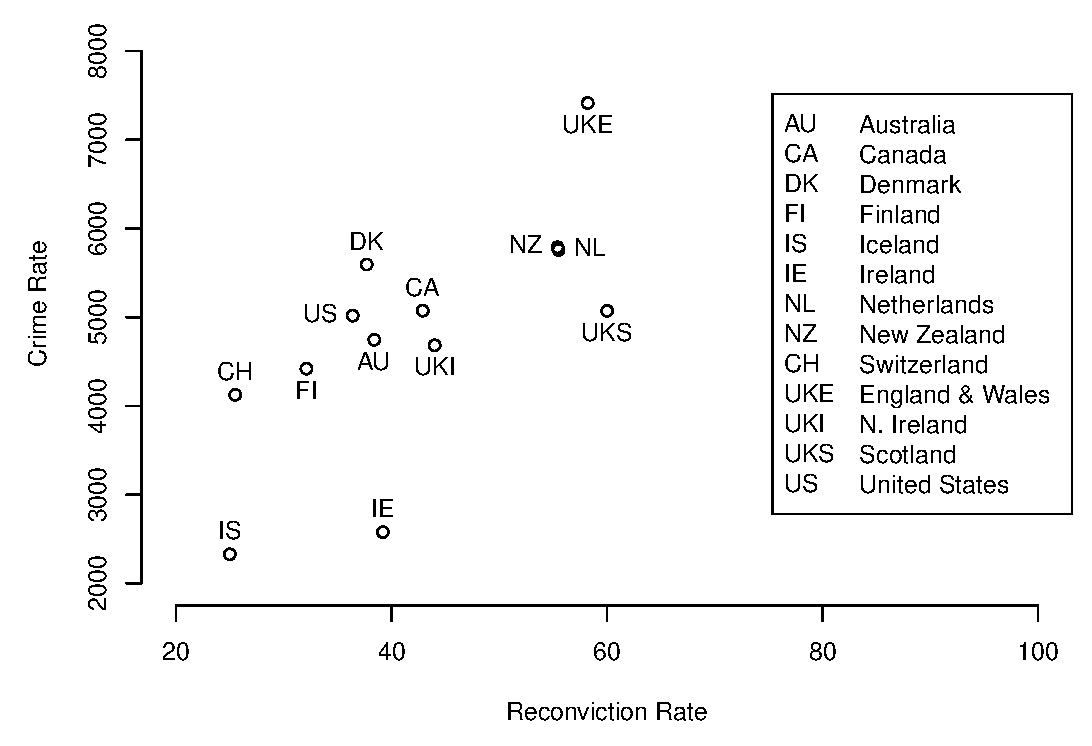
\includegraphics[width=6in, height=3.75in, keepaspectratio=true]{graph303.eps}
\caption{Scatterplot of International Reconviction and Crime Rates}
\end{center}
\end{figure}

The examination of the relationship between international recidivism and crime rates is performed at an elementary level and is purely descriptive in nature.  Table 3.1 indicates that 13 countries reported a 2-year reconviction rate and these countries were used for examining the relationship between recidivism and crime.  A scatterplot for these 13 countries is presented in Figure 3.1.  All of the crime rate statistics are dated to 2003, but the dates for the 2-year reconviction rates vary from country to country.  Because the prisoner release dates for the reconviction statistics tend to be relatively close to 2003 and reconviction rates do not appear to fluctuate radically from year to year, the reconviction rates used to examine the relationship appear reasonably accurate.  Figure 3.1 does not produce any visual evidence that the relationship between recidivism and crime is negative.  More formally, the Pearson correlation coefficient for this relationship is $.6992$ with $p = .007$, which indicates a rather strong positive relationship.  Thus, the evidence appears to contradict Kanazawa's claim that the relationship between recidivism and crime is negative and thereby undermines this particular deterministic theory of recidivism behavior.

%%%%%%%%%%%%%%%%%%%%%%%%%%%%%%%%%%%%%%%%%%%%%%%%%%%%%%%%%%%%%%%%%%%%%%%%%%%%%%%%%%%%%%%%%%%%%%%%%%%%%%%%%%%%%%%%%%%%%
% - THESE ARE THE STATISTICAL RESULTS OF THE CORRELATION TEST
%
%Table 3.1 indicates that 13 countries report a two-year reconviction rate, which is the largest number of observations for any of the follow-up periods.  Thus, the values from these 13 countries will be used for the analysis.  Computation of the correlation coefficient produces the result that $r = .6992$, where $t(11) = 3.2437$ and $p = .0078$ (two-tailed).
%%%%%%%%%%%%%%%%%%%%%%%%%%%%%%%%%%%%%%%%%%%%%%%%%%%%%%%%%%%%%%%%%%%%%%%%%%%%%%%%%%%%%%%%%%%%%%%%%%%%%%%%%%%%%%%%%%%%

The second relationship of interest concerns the crime and incarceration rates.  This relationship is of great importance to criminal justice and corrections policy because its true direction and strength can either support or refute the proposition that incarcerating a greater number of offenders lowers the overall crime rate.  As with the analysis of the previous relationship, the examination of the relationship between crime and incarceration is elementary and purely descriptive.  The statistics for both the crime and incarceration rates are all dated to 2003 for all countries.  All 17 countries are represented in the scatterplot in Figure 3.2.  A fitted line was included to provide a sense of the direction of the numerical relationship.

\begin{figure}[b]
\begin{center}
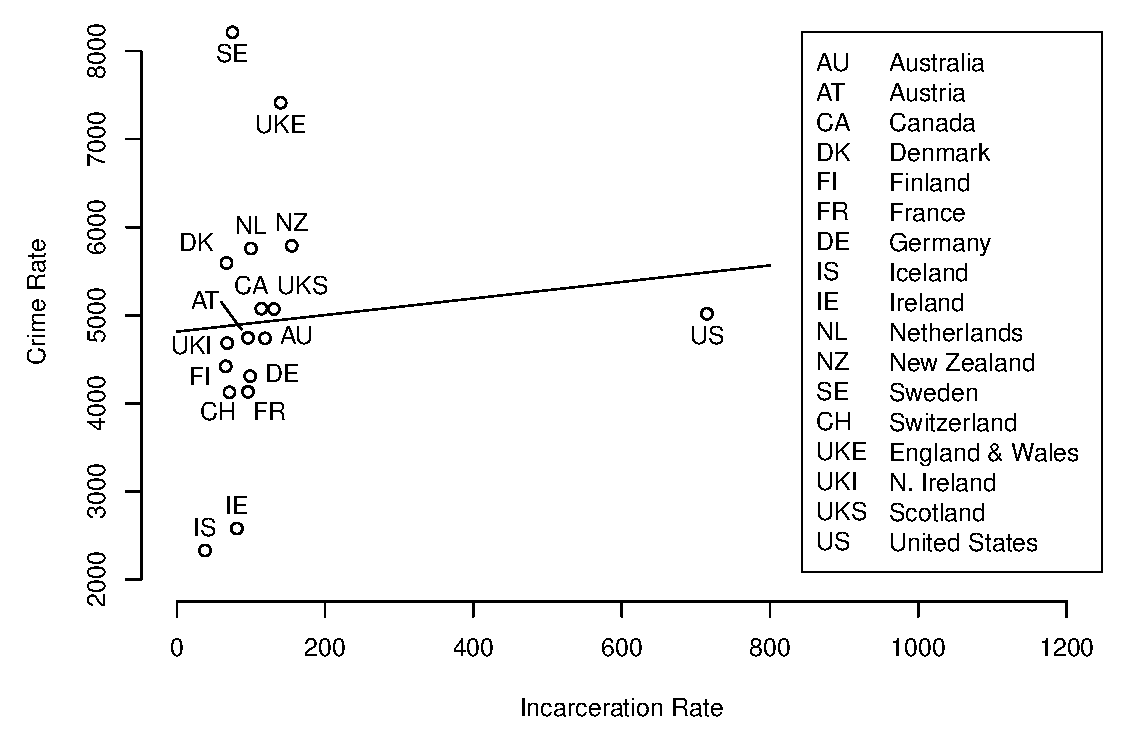
\includegraphics[width=5.9in, height=3.75in, keepaspectratio=true]{graph301c.eps}
\caption{Scatterplot of International Crime and Incarceration Rates}
\end{center}
\end{figure}

As Figure 3.2 makes apparent, one particular country stands out from the rest.  The scatterplot reveals that, in comparison with all of the other countries, the United States has an extremely high incarceration rate.  When the United States is excluded from the calculation, the mean incarceration rate per 100,000 members of the population for the other 16 countries is 94.75.  With an incarceration rate of 715 per 100,000 members of the population, the incarceration rate for the United States is more than seven times the size of the mean incarceration rate for the other 16 countries.

The United States is such an extreme observation that the other observations are consequently compressed in the graph, thereby making it difficult to ascertain the nature of the relationship.  The fitted line reveals that the relationship is slightly positive.  The correlation coefficient is $.0997$ and the probability is very low that a relationship exists at all.  If the United States is excluded, the correlation coefficient is $.4367$ and it is likely that the relationship is, in fact, positive.

% THE CORRELATION TEST RESULTS FOR RELATIONSHIP NO. 2
%
%The analysis of the correlation coefficient that includes the United States produces the following results:  $r = .0997$, where $t(15)=.3883$ and $p=.7033$ (two-tailed).  The suggestion is that no relationship exists between the crime rate and the incarceration rate.  This analysis is given graphical representation as a scatterplot in Figure 3.1, which includes a fitted line representing the statistically insignificant relationship.  Leaving out the United States, the correlation analysis yields the following results:  $r = .4367$, where $t(14)=1.8164$ and $p=.0908$ (two-tailed).  Although the relationship is not exceedingly strong, there does appear to be a positive relationship between the crime and incarceration rates that is statistically significant at the $.1$ level.

%\begin{figure}[t]
%\begin{center}
%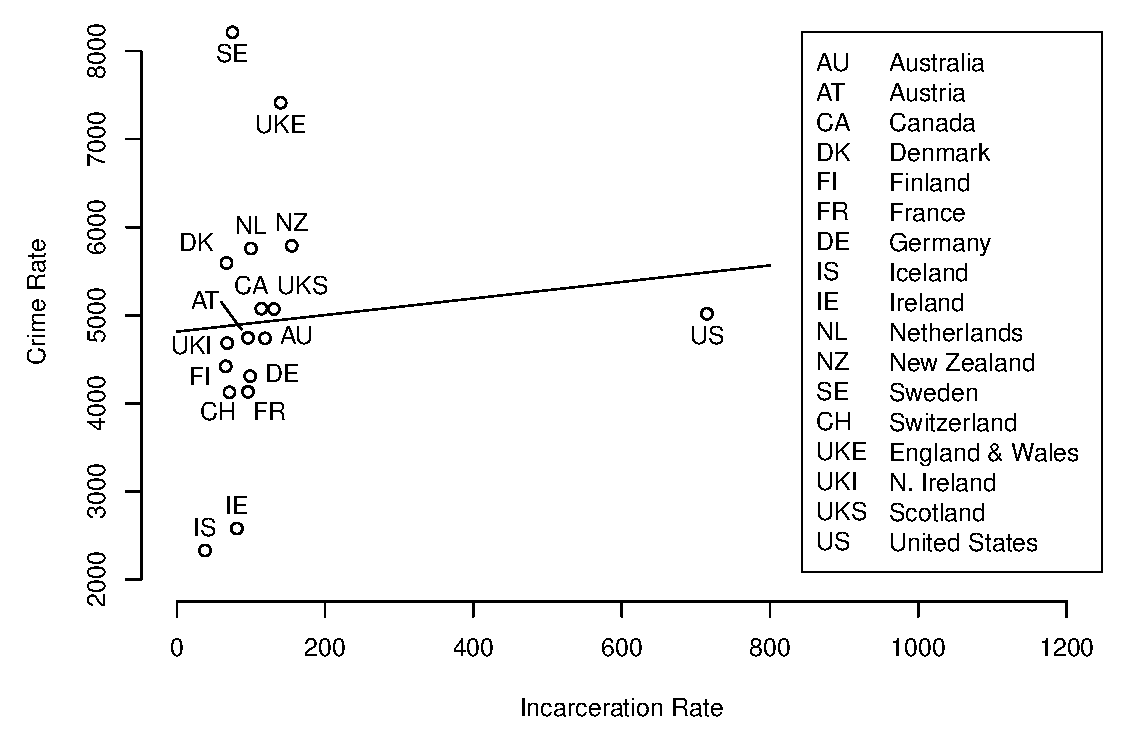
\includegraphics[width=5.9in, height=3.75in, keepaspectratio=true]{graph301c.eps}
%\caption{Scatterplot of International Crime and Incarceration Rates}
%\end{center}
%\end{figure}

This elementary analysis suggests that the policy of attempting to lower the crime rate by imprisoning an ever larger numbers of individuals has no empirical support.  The mean crime rate for all 17 countries is 4,941 per 100,000 members of the population and the United States is very close to the mean with a crime rate of 5,018 per 100,000.  With such a high incarceration rate, if there were any substance to the claim that locking up more prisoners reduces the crime rate, the United States should exhibit a crime rate substantially below the mean.  It would be presumptuous to assert that those who determine criminal justice and corrections policy base their policy decisions on statistical evidence, regardless of what prior statistical evidence might suggest about this particular relationship.  Nevertheless, the high incarceration rate in the United States is likely to find its justification in either a belief that incarcerating more individuals reduces crime or a belief that retribution demands a high level of incarceration.  If the rationale behind locking up large numbers of individuals in prison is the belief that it lowers crime, the evidence does not appear to support this view.  If retribution is the motive behind the high incarceration rate, the satisfaction of this subjective moral belief carries a rather high price in terms of taxpayer dollars.

While the analysis of the relationship between the crime and incarceration rates found above does not constitute a definitive proof of the relationship's qualitative or quantitative properties, it certainly raises questions about justification and efficacy of policies that support increasing the incarceration rate.  Clearly, criminal justice and corrections policy must address two important issues.  First, the relationship between the crime and incarceration rates must be extensively researched to definitively establish its direction and magnitude so as to determine its role within the formation of policy decisions.  Second, a rational, well-informed debate is needed to determine whether the public interest is best served by policies motivated by retribution or policies focusing on public safety and cost minimization.

\section[Evaluating the international standing of the United States]{Evaluating the international standing\\ of the United States}

The absence of standardized, internationally-accepted methods for collecting and analyzing recidivism data makes international comparisons precarious at best.  For two countries, Finland and Ireland, only reincarceration rates were available and these rates had to be interpreted as lower bounds for the reconviction rates.  Scotland's data contains errors in the form of ``pseudo-recidivism,'' reconvictions for crimes committed prior to the initial prison sentences from which the offenders were released.  While the three aforementioned countries put forth rates that were approximations of reconviction rates, some doubt remains as to their overall accuracy.  With the recent appearance of higher quality, nationwide recidivism studies, it appears as though many countries in Europe are moving toward adopting the policy goal of producing annual, standardized recidivism statistics.  At the present, there are still some problems of comparability with respect to international recidivism rates.  These difficulties notwithstanding, the international comparisons of recidivism are viewed here to be reasonably accurate and useful for evaluating how the United States ranks in comparison with other countries exhibiting similar economic, political, and cultural qualities.

\begin{figure}[b]
\begin{center}
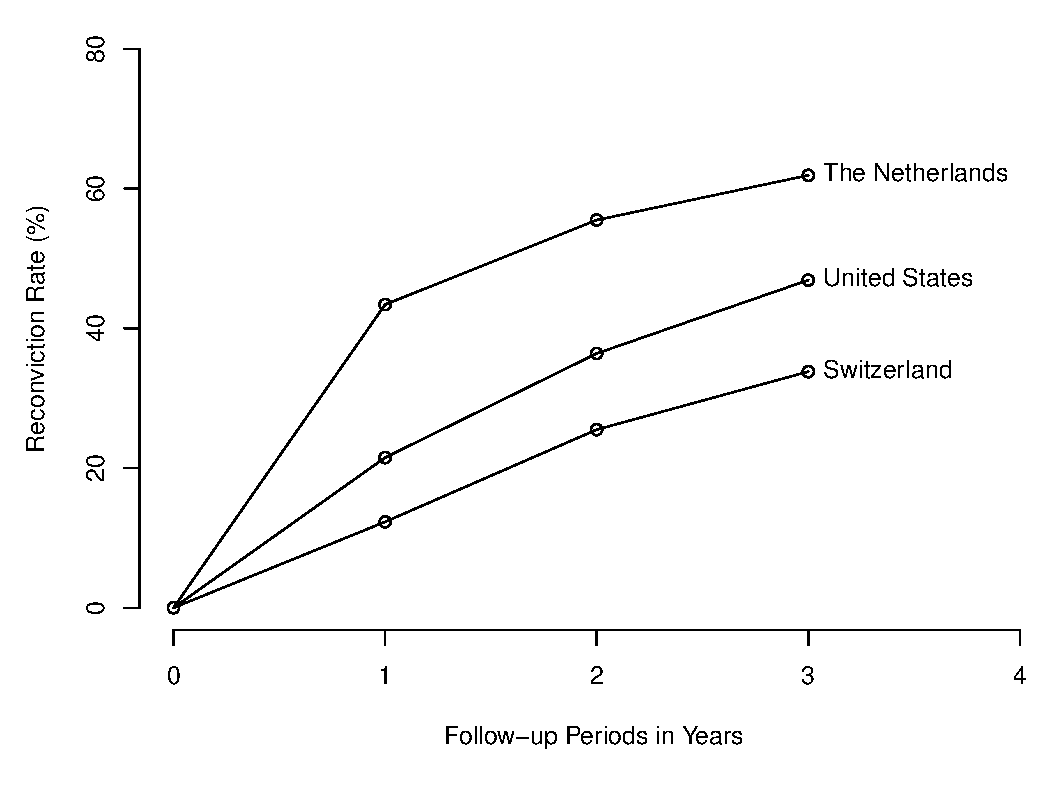
\includegraphics[width=5.9in, height=3.95in, keepaspectratio=true]{graph302b.eps}
\caption{Reconviction Rates for The Netherlands, Switzerland, and the U.S.}
\end{center}
\end{figure}

In summary, the recidivism rate in the United States, measured in terms of the reconviction rate, was found to be slightly lower than the average of the 17 countries in these comparisons.  Figure 3.2 is an accurate graphical representation of where the United States stands in relation to the highest and lowest reconviction rates for the first 3 follow-up years.  Because the recidivism statistics for the Netherlands are of the highest quality, their reconviction rate was used to represent the highest rate.  While Iceland had a slightly lower reconviction rate during the first 2 follow-up years, Switzerland's reconviction rate was chosen to represent the lowest overall rate because its 5-year rate was clearly the lowest for all 17 countries.  In evaluative terms, the United States' recidivism rate compares favorably with most of the selected countries.  No attempts have been made within the literature to determine the lowest recidivism rate that a given society could realistically achieve.  However, the United States' 3-year reconviction rate is 38.8\% larger than that of Switzerland, which suggests that there is room for improvement for the United States.

Besides the international comparisons of recidivism, two relationships between crime, incarceration, and recidivism rates were examined in this chapter.  The first relationship examined was between the crime and recidivism rates and the empirical evidence appears to contradict a deterministic theory that asserts a negative relationship.  Showing that this theory may not have any empirical support is important because it might ultimately change some opinions toward the view that successful rehabilitation and reintegration is still a possibility.  The second relationship considered was between the crime and incarceration rates.  The belief that the crime rate decreases as more criminals are incarcerated implies a negative relationship between these variables.  The evidence indicates that either there is no relationship between these variables or the relationship is, in fact, positive.  In either case, the evidence here does not support the view that increasing the incarceration rate lowers the crime rate.  